% Options for packages loaded elsewhere
\PassOptionsToPackage{unicode}{hyperref}
\PassOptionsToPackage{hyphens}{url}
%
\documentclass[
  ignorenonframetext,
]{beamer}
\usepackage{pgfpages}
\setbeamertemplate{caption}[numbered]
\setbeamertemplate{caption label separator}{: }
\setbeamercolor{caption name}{fg=normal text.fg}
\beamertemplatenavigationsymbolsempty
% Prevent slide breaks in the middle of a paragraph
\widowpenalties 1 10000
\raggedbottom
\setbeamertemplate{part page}{
  \centering
  \begin{beamercolorbox}[sep=16pt,center]{part title}
    \usebeamerfont{part title}\insertpart\par
  \end{beamercolorbox}
}
\setbeamertemplate{section page}{
  \centering
  \begin{beamercolorbox}[sep=12pt,center]{part title}
    \usebeamerfont{section title}\insertsection\par
  \end{beamercolorbox}
}
\setbeamertemplate{subsection page}{
  \centering
  \begin{beamercolorbox}[sep=8pt,center]{part title}
    \usebeamerfont{subsection title}\insertsubsection\par
  \end{beamercolorbox}
}
\AtBeginPart{
  \frame{\partpage}
}
\AtBeginSection{
  \ifbibliography
  \else
    \frame{\sectionpage}
  \fi
}
\AtBeginSubsection{
  \frame{\subsectionpage}
}

\usepackage{amsmath,amssymb}
\usepackage{iftex}
\ifPDFTeX
  \usepackage[T1]{fontenc}
  \usepackage[utf8]{inputenc}
  \usepackage{textcomp} % provide euro and other symbols
\else % if luatex or xetex
  \usepackage{unicode-math}
  \defaultfontfeatures{Scale=MatchLowercase}
  \defaultfontfeatures[\rmfamily]{Ligatures=TeX,Scale=1}
\fi
\usepackage{lmodern}
\ifPDFTeX\else  
    % xetex/luatex font selection
\fi
% Use upquote if available, for straight quotes in verbatim environments
\IfFileExists{upquote.sty}{\usepackage{upquote}}{}
\IfFileExists{microtype.sty}{% use microtype if available
  \usepackage[]{microtype}
  \UseMicrotypeSet[protrusion]{basicmath} % disable protrusion for tt fonts
}{}
\makeatletter
\@ifundefined{KOMAClassName}{% if non-KOMA class
  \IfFileExists{parskip.sty}{%
    \usepackage{parskip}
  }{% else
    \setlength{\parindent}{0pt}
    \setlength{\parskip}{6pt plus 2pt minus 1pt}}
}{% if KOMA class
  \KOMAoptions{parskip=half}}
\makeatother
\usepackage{xcolor}
\newif\ifbibliography
\setlength{\emergencystretch}{3em} % prevent overfull lines
\setcounter{secnumdepth}{-\maxdimen} % remove section numbering


\providecommand{\tightlist}{%
  \setlength{\itemsep}{0pt}\setlength{\parskip}{0pt}}\usepackage{longtable,booktabs,array}
\usepackage{calc} % for calculating minipage widths
\usepackage{caption}
% Make caption package work with longtable
\makeatletter
\def\fnum@table{\tablename~\thetable}
\makeatother
\usepackage{graphicx}
\makeatletter
\def\maxwidth{\ifdim\Gin@nat@width>\linewidth\linewidth\else\Gin@nat@width\fi}
\def\maxheight{\ifdim\Gin@nat@height>\textheight\textheight\else\Gin@nat@height\fi}
\makeatother
% Scale images if necessary, so that they will not overflow the page
% margins by default, and it is still possible to overwrite the defaults
% using explicit options in \includegraphics[width, height, ...]{}
\setkeys{Gin}{width=\maxwidth,height=\maxheight,keepaspectratio}
% Set default figure placement to htbp
\makeatletter
\def\fps@figure{htbp}
\makeatother

\makeatletter
\@ifpackageloaded{tcolorbox}{}{\usepackage[skins,breakable]{tcolorbox}}
\@ifpackageloaded{fontawesome5}{}{\usepackage{fontawesome5}}
\definecolor{quarto-callout-color}{HTML}{909090}
\definecolor{quarto-callout-note-color}{HTML}{0758E5}
\definecolor{quarto-callout-important-color}{HTML}{CC1914}
\definecolor{quarto-callout-warning-color}{HTML}{EB9113}
\definecolor{quarto-callout-tip-color}{HTML}{00A047}
\definecolor{quarto-callout-caution-color}{HTML}{FC5300}
\definecolor{quarto-callout-color-frame}{HTML}{acacac}
\definecolor{quarto-callout-note-color-frame}{HTML}{4582ec}
\definecolor{quarto-callout-important-color-frame}{HTML}{d9534f}
\definecolor{quarto-callout-warning-color-frame}{HTML}{f0ad4e}
\definecolor{quarto-callout-tip-color-frame}{HTML}{02b875}
\definecolor{quarto-callout-caution-color-frame}{HTML}{fd7e14}
\makeatother
\makeatletter
\makeatother
\makeatletter
\makeatother
\makeatletter
\@ifpackageloaded{caption}{}{\usepackage{caption}}
\AtBeginDocument{%
\ifdefined\contentsname
  \renewcommand*\contentsname{Table of contents}
\else
  \newcommand\contentsname{Table of contents}
\fi
\ifdefined\listfigurename
  \renewcommand*\listfigurename{List of Figures}
\else
  \newcommand\listfigurename{List of Figures}
\fi
\ifdefined\listtablename
  \renewcommand*\listtablename{List of Tables}
\else
  \newcommand\listtablename{List of Tables}
\fi
\ifdefined\figurename
  \renewcommand*\figurename{Figure}
\else
  \newcommand\figurename{Figure}
\fi
\ifdefined\tablename
  \renewcommand*\tablename{Table}
\else
  \newcommand\tablename{Table}
\fi
}
\@ifpackageloaded{float}{}{\usepackage{float}}
\floatstyle{ruled}
\@ifundefined{c@chapter}{\newfloat{codelisting}{h}{lop}}{\newfloat{codelisting}{h}{lop}[chapter]}
\floatname{codelisting}{Listing}
\newcommand*\listoflistings{\listof{codelisting}{List of Listings}}
\makeatother
\makeatletter
\@ifpackageloaded{caption}{}{\usepackage{caption}}
\@ifpackageloaded{subcaption}{}{\usepackage{subcaption}}
\makeatother
\makeatletter
\@ifpackageloaded{tcolorbox}{}{\usepackage[skins,breakable]{tcolorbox}}
\makeatother
\makeatletter
\@ifundefined{shadecolor}{\definecolor{shadecolor}{rgb}{.97, .97, .97}}
\makeatother
\makeatletter
\makeatother
\makeatletter
\makeatother
\ifLuaTeX
  \usepackage{selnolig}  % disable illegal ligatures
\fi
\IfFileExists{bookmark.sty}{\usepackage{bookmark}}{\usepackage{hyperref}}
\IfFileExists{xurl.sty}{\usepackage{xurl}}{} % add URL line breaks if available
\urlstyle{same} % disable monospaced font for URLs
\hypersetup{
  pdftitle={Santé et Démocratie},
  pdfauthor={Olivier Caron},
  hidelinks,
  pdfcreator={LaTeX via pandoc}}

\title{Santé et Démocratie}
\subtitle{Etudes démocratiques}
\author{Olivier Caron}
\date{January 17, 2025}

\begin{document}
\frame{\titlepage}
\ifdefined\Shaded\renewenvironment{Shaded}{\begin{tcolorbox}[enhanced, interior hidden, breakable, borderline west={3pt}{0pt}{shadecolor}, frame hidden, sharp corners, boxrule=0pt]}{\end{tcolorbox}}\fi

\begin{frame}{Intervenants : Jean-François Delfraissy}
\protect\hypertarget{intervenants-jean-franuxe7ois-delfraissy}{}
Président du CCNE (Comité Consultatif National d'Éthique), Paris-Saclay
\end{frame}

\begin{frame}{\textbf{Michel Foucault -- \emph{Il faut défendre la
société}}}
\protect\hypertarget{michel-foucault-il-faut-duxe9fendre-la-sociuxe9tuxe9}{}
\begin{itemize}
\tightlist
\item
  La médecine dépasse le cadre strictement médical : elle comporte un
  \textbf{aspect politique} complexe, notamment en période de crise
  sanitaire.\\
\item
  \textbf{Biopouvoir} : Concept développé par Michel Foucault, qui
  souligne que :

  \begin{itemize}
  \tightlist
  \item
    Le pouvoir sur la vie (santé, corps) ne doit pas être monopolisé par
    les institutions ou les médecins.\\
  \item
    La maladie \textbf{appartient au malade}, non au médecin.\\
  \item
    Le rôle du médecin est d'agir comme une \textbf{boussole}, guidant
    le patient/citoyen, sans exercer de contrôle autoritaire.\\
  \end{itemize}
\item
  Ce concept prend une importance particulière dans le contexte des
  \textbf{années sida}, remettant en question la nature même du
  biopouvoir.
\end{itemize}
\end{frame}

\begin{frame}{\textbf{Quelques grandes vérités sur la médecine}}
\protect\hypertarget{quelques-grandes-vuxe9rituxe9s-sur-la-muxe9decine}{}
\begin{block}{1. \textbf{Santé et contexte global}}
\protect\hypertarget{santuxe9-et-contexte-global}{}
\begin{itemize}
\tightlist
\item
  La santé ne peut être dissociée de ses \textbf{déterminants globaux} :

  \begin{itemize}
  \tightlist
  \item
    Société, environnement, nutrition, modes de vie.
  \item
    Exemples :

    \begin{itemize}
    \tightlist
    \item
      Environnement social (conditions de vie).\\
    \item
      Habitudes personnelles (tabac, activité physique, alimentation).
    \end{itemize}
  \end{itemize}
\end{itemize}
\end{block}

\begin{block}{2. \textbf{Chiffres clés}}
\protect\hypertarget{chiffres-cluxe9s}{}
\begin{itemize}
\tightlist
\item
  \textbf{20\%} de la santé est directement liée à la \textbf{médecine
  de soins}.\\
\item
  \textbf{80\%} des déterminants de la santé sont sociétaux et
  comportementaux :

  \begin{itemize}
  \tightlist
  \item
    Exemples : arrêter de fumer, marcher 10 000 pas par jour, avoir une
    alimentation équilibrée.\\
  \end{itemize}
\item
  Pourtant, \textbf{90\% des budgets} en santé sont alloués aux
  \textbf{soins}, laissant peu de place à la prévention.

  \begin{itemize}
  \tightlist
  \item
    Cela crée une \textbf{incohérence majeure} dans les politiques de
    santé publique.
  \end{itemize}
\end{itemize}
\end{block}

\begin{block}{3. \textbf{Prévention insuffisante}}
\protect\hypertarget{pruxe9vention-insuffisante}{}
\begin{itemize}
\tightlist
\item
  La prévention est sous-financée et mal coordonnée :

  \begin{itemize}
  \tightlist
  \item
    \textbf{Manque de budget} pour les campagnes préventives.\\
  \item
    Faible implication des acteurs locaux et associatifs.
  \end{itemize}
\end{itemize}
\end{block}

\begin{block}{4. \textbf{Santé et citoyenneté}}
\protect\hypertarget{santuxe9-et-citoyennetuxe9}{}
\begin{itemize}
\tightlist
\item
  La santé \textbf{n'appartient ni aux médecins ni aux politiques}, mais
  \textbf{aux citoyens}.

  \begin{itemize}
  \tightlist
  \item
    Cela implique une démocratisation des débats et des décisions liés à
    la santé.\\
  \item
    L'\textbf{éthique du soin} devient un enjeu \textbf{citoyen}.\\
  \item
    Les \textbf{milieux associatifs} doivent jouer un rôle
    \textbf{majeur} pour mobiliser et représenter les citoyens.
  \end{itemize}
\end{itemize}
\end{block}
\end{frame}

\begin{frame}{\textbf{Évolution des connaissances médicales}}
\protect\hypertarget{uxe9volution-des-connaissances-muxe9dicales}{}
\begin{itemize}
\tightlist
\item
  La \textbf{demi-vie des connaissances médicales} est estimée à
  \textbf{2 ans}, soulignant la rapidité des progrès scientifiques.\\
\item
  Ce renouvellement constant ouvre des perspectives, même dans des
  domaines autrefois perçus comme des ``plafonds de verre'' :

  \begin{itemize}
  \tightlist
  \item
    Exemple : Recherche sur Alzheimer et d'autres maladies
    dégénératives.
  \end{itemize}
\end{itemize}
\end{frame}

\begin{frame}
\begin{tcolorbox}[enhanced jigsaw, rightrule=.15mm, opacityback=0, colframe=quarto-callout-important-color-frame, bottomtitle=1mm, toptitle=1mm, left=2mm, leftrule=.75mm, title=\textcolor{quarto-callout-important-color}{\faExclamation}\hspace{0.5em}{À retenir :}, toprule=.15mm, breakable, colback=white, coltitle=black, opacitybacktitle=0.6, titlerule=0mm, bottomrule=.15mm, colbacktitle=quarto-callout-important-color!10!white, arc=.35mm]

\begin{enumerate}
\tightlist
\item
  \textbf{La santé est bien plus que le soin.}\\
\item
  \textbf{La maladie appartient au malade, pas au médecin.}\\
\end{enumerate}

\end{tcolorbox}
\end{frame}

\begin{frame}{Émergence infectieuse : une constante répétition}
\protect\hypertarget{uxe9mergence-infectieuse-une-constante-ruxe9puxe9tition}{}
\begin{block}{Exemples récents de pandémies ou d'épidémies majeures :}
\protect\hypertarget{exemples-ruxe9cents-de-panduxe9mies-ou-duxe9piduxe9mies-majeures}{}
\begin{itemize}
\tightlist
\item
  \textbf{SARS} : 2003\\
\item
  \textbf{Chikungunya} : 2005\\
\item
  \textbf{H1N1 (Grippe A)} : 2009\\
\item
  \textbf{MERS-CoV} : 2013\\
\item
  \textbf{Ebola} : 2014\\
\item
  \textbf{Zika} : 2015\\
\item
  \textbf{SARS-CoV-2 (Covid-19)} :

  \begin{itemize}
  \tightlist
  \item
    Durée : \textbf{2020-2022}
  \end{itemize}
\end{itemize}
\end{block}
\end{frame}

\begin{frame}
\begin{block}{Facteurs majeurs favorisant l'émergence infectieuse :}
\protect\hypertarget{facteurs-majeurs-favorisant-luxe9mergence-infectieuse}{}
\begin{enumerate}
\tightlist
\item
  \textbf{Changements climatiques et du monde vivant} :

  \begin{itemize}
  \tightlist
  \item
    Modification des écosystèmes (déforestation, perte de
    biodiversité).\\
  \item
    Apparition de nouveaux réservoirs ou vecteurs (ex. moustiques).
  \end{itemize}
\item
  \textbf{Changements démographiques et répartition des populations} :

  \begin{itemize}
  \tightlist
  \item
    Urbanisation croissante et surpopulation.\\
  \item
    Mobilité humaine accrue (migrations, voyages internationaux).
  \end{itemize}
\item
  \textbf{Changements technologiques et interactions humaines} :

  \begin{itemize}
  \tightlist
  \item
    Intensification des échanges mondiaux.\\
  \item
    Interactions accrues entre humains, animaux domestiques et sauvages.
  \end{itemize}
\end{enumerate}
\end{block}

\begin{block}{Sources :}
\protect\hypertarget{sources}{}
\begin{itemize}
\tightlist
\item
  \textbf{Baker et al.}, \emph{Nature Reviews}, 2021\\
\item
  \textbf{T. Lefrançois}, \emph{The Lancet}, 2022
\end{itemize}
\end{block}
\end{frame}

\begin{frame}
\begin{tcolorbox}[enhanced jigsaw, rightrule=.15mm, opacityback=0, colframe=quarto-callout-important-color-frame, bottomtitle=1mm, toptitle=1mm, left=2mm, leftrule=.75mm, title=\textcolor{quarto-callout-important-color}{\faExclamation}\hspace{0.5em}{Les 3 grandes menaces à surveiller pour les années à venir :}, toprule=.15mm, breakable, colback=white, coltitle=black, opacitybacktitle=0.6, titlerule=0mm, bottomrule=.15mm, colbacktitle=quarto-callout-important-color!10!white, arc=.35mm]

\begin{enumerate}
\tightlist
\item
  \textbf{Maladies infectieuses} : Émergences potentielles de nouvelles
  épidémies/pandémies.\\
\item
  \textbf{Malbouffe} : Impacts sur les maladies chroniques (diabète,
  obésité, etc.).\\
\item
  \textbf{Vieillissement de la population} : Enjeux économiques, sociaux
  et sanitaires liés à la longévité croissante.\\
\end{enumerate}

\end{tcolorbox}
\end{frame}

\begin{frame}{Le Nil -- Égypte (1968-2018)}
\protect\hypertarget{le-nil-uxe9gypte-1968-2018}{}
\begin{block}{Contexte historique}
\protect\hypertarget{contexte-historique}{}
\begin{itemize}
\tightlist
\item
  \textbf{1967} : Guerre des Six Jours (conflit israélo-arabe) :

  \begin{itemize}
  \tightlist
  \item
    Défaite militaire de l'Égypte face à Israël.
  \item
    Déstabilisation politique majeure : le président \textbf{Gamal Abdel
    Nasser}, leader du panarabisme, annonce sa démission le \textbf{9
    juin 1967}. Sous la pression populaire, il revient au pouvoir peu
    après.
  \end{itemize}
\end{itemize}
\end{block}
\end{frame}

\begin{frame}
\begin{block}{Transformations du Nil (1968-2018)}
\protect\hypertarget{transformations-du-nil-1968-2018}{}
\begin{block}{1. \textbf{Le rôle du Nil dans le développement égyptien}}
\protect\hypertarget{le-ruxf4le-du-nil-dans-le-duxe9veloppement-uxe9gyptien}{}
\begin{itemize}
\tightlist
\item
  Le Nil, source vitale pour l'Égypte, représente :

  \begin{itemize}
  \tightlist
  \item
    \textbf{97\% de l'approvisionnement en eau douce} du pays.
  \item
    Une ressource essentielle pour l'agriculture, l'énergie
    hydroélectrique, et la survie de la population.
  \end{itemize}
\end{itemize}
\end{block}

\begin{block}{2. \textbf{Projets de gestion de l'eau}}
\protect\hypertarget{projets-de-gestion-de-leau}{}
\begin{itemize}
\tightlist
\item
  Construction du \textbf{barrage d'Assouan} (terminé en 1970, initié
  sous Nasser) :

  \begin{itemize}
  \tightlist
  \item
    Permet un meilleur contrôle des crues et une irrigation stable.
  \item
    Fournit une importante source d'énergie via l'hydroélectricité.
  \item
    \textbf{Conséquences négatives} :

    \begin{itemize}
    \tightlist
    \item
      Perte de fertilité des sols en aval.
    \item
      Érosion de la biodiversité dans le delta du Nil.
    \end{itemize}
  \end{itemize}
\end{itemize}
\end{block}

\begin{block}{3. \textbf{Défis contemporains}}
\protect\hypertarget{duxe9fis-contemporains}{}
\begin{itemize}
\tightlist
\item
  \textbf{Croissance démographique} : La population égyptienne passe de
  30 millions en 1968 à près de 100 millions en 2018, augmentant la
  pression sur les ressources en eau.
\item
  \textbf{Tensions hydropolitiques} :

  \begin{itemize}
  \tightlist
  \item
    Construction du \textbf{Grand Barrage de la Renaissance} par
    l'Éthiopie (2011-2020), suscitant des différends sur le partage des
    eaux du Nil.
  \item
    Négociations complexes entre l'Égypte, le Soudan et l'Éthiopie.
  \end{itemize}
\end{itemize}
\end{block}

\begin{block}{4. \textbf{Changement climatique}}
\protect\hypertarget{changement-climatique}{}
\begin{itemize}
\tightlist
\item
  Réduction des précipitations et montée du niveau de la mer affectant
  le delta du Nil.
\item
  Salinisation croissante des terres agricoles en aval, menaçant la
  sécurité alimentaire. \#\# Le Fleuve Sénégal
\end{itemize}
\end{block}
\end{block}

\begin{block}{Années 1980 -- Saint-Louis, Sénégal}
\protect\hypertarget{annuxe9es-1980-saint-louis-suxe9nuxe9gal}{}
\begin{itemize}
\tightlist
\item
  \textbf{Impact des barrages} :

  \begin{itemize}
  \tightlist
  \item
    La construction des barrages de \textbf{Diama} et \textbf{Manantali}
    entraîne une diminution de la salinité de l'eau dans la région.
  \item
    Conséquences positives :

    \begin{itemize}
    \tightlist
    \item
      Développement agricole grâce à des zones cultivées riches en
      légumes (+++).
    \item
      Amélioration économique de la région.
    \end{itemize}
  \item
    Conséquences négatives :

    \begin{itemize}
    \tightlist
    \item
      Apparition de la \textbf{bilharziose urinaire} due à
      \emph{Schistosoma haematobium} :

      \begin{itemize}
      \tightlist
      \item
        La baisse de la salinité de l'eau favorise la prolifération des
        escargots hôtes du parasite.
      \item
        Les enfants, malgré les avertissements, continuent de jouer dans
        l'eau contaminée.
      \end{itemize}
    \item
      Le gouvernement sénégalais exprime son inquiétude : bien que le
      développement économique soit important, ce problème de santé
      publique représente un \textbf{gros danger}.
    \end{itemize}
  \end{itemize}
\end{itemize}
\end{block}
\end{frame}

\begin{frame}
\begin{block}{Le vaccin contre la bilharziose}
\protect\hypertarget{le-vaccin-contre-la-bilharziose}{}
\begin{itemize}
\tightlist
\item
  \textbf{Développement du vaccin (1993-2012)} :

  \begin{itemize}
  \tightlist
  \item
    Mené par l'équipe d'\textbf{André et Monique Capron} à Lille.
  \item
    Objectif : créer un vaccin efficace pour lutter contre
    \emph{Schistosoma haematobium}.
  \item
    Les essais sont suivis avec beaucoup d'espoir. Le vaccin est censé
    ``fonctionner''.
  \end{itemize}
\item
  \textbf{Résultats décevants en 2012} :

  \begin{itemize}
  \tightlist
  \item
    Les essais contrôlés randomisés montrent que le vaccin n'a
    \textbf{aucun effet}.
  \item
    Le professeur, chargé d'analyser les données, annonce ces résultats
    aux autorités.
  \item
    Réaction des autorités :

    \begin{itemize}
    \tightlist
    \item
      Le Premier ministre, dépité par les résultats, envisage malgré
      tout de déclarer publiquement que le vaccin fonctionne pour ne pas
      briser l'espoir ou compromettre les investissements.
    \end{itemize}
  \end{itemize}
\end{itemize}
\end{block}
\end{frame}

\begin{frame}
\begin{block}{Défi : Comment expliquer un résultat négatif aux autorités
?}
\protect\hypertarget{duxe9fi-comment-expliquer-un-ruxe9sultat-nuxe9gatif-aux-autorituxe9s}{}
\begin{itemize}
\tightlist
\item
  Importance de communiquer clairement sur la \textbf{science et les
  limites des interventions} :

  \begin{itemize}
  \tightlist
  \item
    Éviter de céder à la pression politique ou économique.
  \item
    Préserver l'intégrité scientifique tout en proposant des solutions
    alternatives pour répondre à la crise sanitaire.
  \end{itemize}
\item
  Le cas met en lumière les tensions entre :

  \begin{itemize}
  \tightlist
  \item
    Les \textbf{exigences politiques} (maintenir une image positive et
    rassurer la population).
  \item
    Les \textbf{réalités scientifiques} (accepter et tirer des leçons
    des échecs).
  \end{itemize}
\end{itemize}
\end{block}
\end{frame}

\begin{frame}{Afrique du Sud (1996-2006)}
\protect\hypertarget{afrique-du-sud-1996-2006}{}
\begin{block}{Contexte général}
\protect\hypertarget{contexte-guxe9nuxe9ral}{}
\begin{itemize}
\tightlist
\item
  \textbf{VIH en Afrique du Sud} :

  \begin{itemize}
  \tightlist
  \item
    Le pays est le plus touché au monde par le VIH dès \textbf{1988}.
  \item
    En \textbf{1996}, l'arrivée de la \textbf{trithérapie} marque une
    avancée majeure : bien que le VIH ne soit toujours pas éradiqué, la
    trithérapie permet d'atténuer considérablement ses effets.
  \end{itemize}
\end{itemize}
\end{block}

\begin{block}{Le rôle controversé du Ministère de la Santé}
\protect\hypertarget{le-ruxf4le-controversuxe9-du-ministuxe8re-de-la-santuxe9}{}
\begin{itemize}
\tightlist
\item
  \textbf{Manto Tshabalala-Msimang} (surnommée ``Dr Betterave'') :

  \begin{itemize}
  \tightlist
  \item
    Ministre de la Santé entre \textbf{1999 et 2008}, elle nie
    l'existence du VIH et refuse de promouvoir les traitements
    antirétroviraux (ARVs).
  \item
    Elle prône une approche basée sur la \textbf{nutrition},
    encourageant les malades à manger des \textbf{betteraves}, de l'ail
    et du citron.
  \item
    Ses positions reflètent le contexte post-apartheid, marqué par une
    méfiance envers les pays occidentaux (``les Blancs du Nord'') et
    leur ingérence perçue.
  \end{itemize}
\end{itemize}
\end{block}

\begin{block}{Conférence de Durban -- 2000}
\protect\hypertarget{confuxe9rence-de-durban-2000}{}
\begin{itemize}
\tightlist
\item
  Lors de la conférence internationale sur le sida à Durban, un moment
  marquant se produit :

  \begin{itemize}
  \tightlist
  \item
    \textbf{Edwin Cameron}, juge blanc et membre de la Cour
    constitutionnelle sud-africaine, affirme publiquement son
    \textbf{homosexualité} et sa \textbf{séropositivité}.
  \item
    Il plaide pour un accès élargi aux \textbf{médicaments
    antirétroviraux}, déclarant qu'il est crucial que l'Afrique prenne
    des mesures.
  \end{itemize}
\end{itemize}
\end{block}

\begin{block}{Conséquences des politiques anti-ARVs}
\protect\hypertarget{consuxe9quences-des-politiques-anti-arvs}{}
\begin{itemize}
\tightlist
\item
  Refus du ministère d'adopter les ARVs :

  \begin{itemize}
  \tightlist
  \item
    Environ \textbf{500 000 morts prématurées} entre 1999 et 2005 sont
    attribuées à cette décision.
  \item
    \textbf{Transmission materno-fœtale} élevée : des millions d'enfants
    naissent contaminés par le VIH.
  \end{itemize}
\end{itemize}
\end{block}

\begin{block}{Acteurs externes et changement}
\protect\hypertarget{acteurs-externes-et-changement}{}
\begin{itemize}
\tightlist
\item
  \textbf{Débat international} :

  \begin{itemize}
  \tightlist
  \item
    Implication d'organisations comme l'\textbf{ANRS} (France) et le
    \textbf{Fonds mondial} pour le financement des trithérapies.
  \end{itemize}
\item
  \textbf{Rôle des entreprises minières} :

  \begin{itemize}
  \tightlist
  \item
    Face à une mortalité élevée parmi leurs jeunes ouvriers, les grandes
    entreprises minières prennent les devants :

    \begin{itemize}
    \tightlist
    \item
      Elles achètent des \textbf{ARVs} et facilitent leur distribution
      parmi leurs employés.
    \item
      Ce tournant marque une amélioration progressive dans la lutte
      contre le VIH en Afrique du Sud.
    \end{itemize}
  \end{itemize}
\end{itemize}
\end{block}
\end{frame}

\begin{frame}{Guinée -- Automne 2014}
\protect\hypertarget{guinuxe9e-automne-2014}{}
\begin{block}{Été 2014}
\protect\hypertarget{uxe9tuxe9-2014}{}
\begin{itemize}
\tightlist
\item
  \textbf{Enterrements} :

  \begin{itemize}
  \tightlist
  \item
    En Guinée, les enterrements doivent être réalisés dans les
    \textbf{48 heures} suivant le décès, selon les traditions
    musulmanes.
  \item
    Les proches touchent les corps des défunts dans le cadre des rites
    religieux/traditionnels, ce qui favorise la propagation de maladies.
  \end{itemize}
\item
  \textbf{Épidémie d'Ebola} :

  \begin{itemize}
  \tightlist
  \item
    Une \textbf{panique générale} s'installe dans la région.
  \item
    La France intervient pour soutenir la Guinée dans la lutte contre
    Ebola.
  \item
    Le professeur (mentionné dans le cours) participait à une
    \textbf{mission interministérielle}.
  \end{itemize}
\item
  \textbf{Institutions impliquées} :

  \begin{itemize}
  \tightlist
  \item
    ANRS (Agence nationale de recherche sur le sida et les hépatites
    virales) et INSERM (Institut national de la santé et de la recherche
    médicale).
  \end{itemize}
\end{itemize}
\end{block}
\end{frame}

\begin{frame}
\begin{block}{Facteurs de propagation}
\protect\hypertarget{facteurs-de-propagation}{}
\begin{itemize}
\tightlist
\item
  \textbf{Pratiques funéraires} :

  \begin{itemize}
  \tightlist
  \item
    Enterrements fréquents (+++) dans les milieux musulmans.
  \item
    Utilisation de \textbf{fosses communes} et de \textbf{linceuls en
    sacs plastiques blancs} comme mesure sanitaire.
  \end{itemize}
\item
  \textbf{Conflits sociaux} :

  \begin{itemize}
  \tightlist
  \item
    Les ONG intervenant dans les villages sont souvent \textbf{mal
    accueillies} et parfois même \textbf{caillassées}.

    \begin{itemize}
    \tightlist
    \item
      \textbf{Conflit} : Les mesures sanitaires imposées (fosses
      communes, interdiction de toucher les corps) sont perçues comme
      une violation des traditions.
    \end{itemize}
  \item
    Le président \textbf{Alpha Condé} refuse d'intervenir directement,
    préférant une approche concertée.
  \end{itemize}
\end{itemize}
\end{block}
\end{frame}

\begin{frame}
\begin{block}{Réponse et adaptation}
\protect\hypertarget{ruxe9ponse-et-adaptation}{}
\begin{itemize}
\tightlist
\item
  \textbf{Communication adaptée} :

  \begin{itemize}
  \tightlist
  \item
    Les ONG ont compris qu'il fallait \textbf{adapter leur discours}
    pour être acceptées.
  \item
    Les \textbf{imams} locaux ont été identifiés comme des relais
    essentiels pour faire passer les messages de santé publique.

    \begin{itemize}
    \tightlist
    \item
      Contrairement au christianisme, l'islam en Guinée n'a pas de
      hiérarchie formelle (pas d'archevêque, d'évêque, etc.).
    \item
      Un \textbf{imam local} d'un petit village peut avoir \textbf{plus
      d'influence} que l'imam de Conakry.
    \end{itemize}
  \end{itemize}
\item
  \textbf{Stratégie} :

  \begin{itemize}
  \tightlist
  \item
    Les imams influents ont été \textbf{réunis et formés} pour expliquer
    les enjeux sanitaires liés à Ebola.
  \item
    Cela a permis de concilier la \textbf{préservation des traditions}
    avec les \textbf{mesures de lutte contre l'épidémie}.
  \end{itemize}
\end{itemize}
\end{block}
\end{frame}

\begin{frame}{Conclusions Provisoires}
\protect\hypertarget{conclusions-provisoires}{}
\begin{enumerate}
\tightlist
\item
  \textbf{Des exemples très réducteurs : une relecture de l'histoire
  \emph{a posteriori}}

  \begin{itemize}
  \tightlist
  \item
    \textbf{Rôle de la médecine} : Elle ne représente que \textbf{25\%
    des bénéfices en santé}, d'autres facteurs jouent un rôle crucial.\\
  \item
    \textbf{Mesures de santé publique} : De nombreuses décisions
    politiques ont eu un impact positif sur la santé publique :

    \begin{itemize}
    \tightlist
    \item
      Feux rouges (sécurité routière)\\
    \item
      Port de la ceinture de sécurité\\
    \item
      Lutte contre le tabac\\
    \item
      Introduction du Nutri-Score pour améliorer l'alimentation\\
    \item
      Campagnes de vaccination
    \end{itemize}
  \end{itemize}
\item
  \textbf{Les dérives potentielles de la médecine dans un contexte
  politique}

  \begin{itemize}
  \tightlist
  \item
    Exemple historique : \textbf{Procès de Nuremberg}, où la médecine a
    été utilisée à des fins idéologiques et politiques, illustrant les
    dangers d'une instrumentalisation scientifique.
  \end{itemize}
\item
  \textbf{Comment s'appuyer sur la science dans des crises
  contemporaines ?}

  \begin{itemize}
  \tightlist
  \item
    Le \textbf{Covid-19} a mis en lumière les défis liés à l'utilisation
    de la science pour orienter les politiques publiques :

    \begin{itemize}
    \tightlist
    \item
      Gestion des incertitudes scientifiques\\
    \item
      Communication auprès du public\\
    \item
      Équilibre entre décisions politiques et recommandations
      scientifiques.
    \end{itemize}
  \end{itemize}
\end{enumerate}
\end{frame}

\begin{frame}{Covid19 en France}
\protect\hypertarget{covid19-en-france}{}
\begin{block}{2020 : Les confinements}
\protect\hypertarget{les-confinements}{}
Premières vague

24 janvier 2020

14 février 2020

10 mars 2020 Création du conseil scientifiques covid

du 17 mars au 11 ma 2020 premier confinement général =\textgreater{} on
commence à mettre les masques et on ccmprend un peu mieux. Le virus est
aussi transmis par les personnes asymptomatiques

juin 2020 Nouvelles contamination \textless5000 par jour

2 juin 2020 StopCOVID application de suivi des contactes

Seconde vague

27 juillet 2020 avis du CS covid19 : une seconde vague prévue à
l'automne si les mesures barrières ne ont pa respctées

Septembre 2020 Reprise épidémique

22 octobre 220 evolution de StopCOVID en TousantiCOVID

29 octobre 2020 : second confinement général (adapté)

10 dévembre 2020: anonce d'un déconfinement progressif par le premier
ministre à partir du 15 décembre 2020 commencant par un couvre feu

2 confinements, couvres feux, pa de vaccin, pas de variant, 65000 décès,
28000 en EHPAD
\end{block}

\begin{block}{2021 : Vaccins et variants}
\protect\hypertarget{vaccins-et-variants}{}
\begin{block}{Troisième vague variant alpha}
\protect\hypertarget{troisiuxe8me-vague-variant-alpha}{}
Fin décembre 2020 un nouveau variant séquence détecté au RU plus
transmissible et létal devient dominannt en France

29 janvier 2021 alerte du conseil scientifque COVID

3 avril 2021 Troisième confinement national Course entre vaccination et
variants

Taux d'occupation des lits de réanimation : 106\% (mettre en rouge le
chiffre)\\
Début mai 2021 : début de sortie de confinement progressif: baisse des
nouvelles contaminations = 20 000 par jour

45k décès
\end{block}

\begin{block}{4è, 5è, et 6è vague (indice è en haut) variant DELTA}
\protect\hypertarget{uxe8-5uxe8-et-6uxe8-vague-indice-uxe8-en-haut-variant-delta}{}
31 mai 2021 : ouverture de la vaccination à tous les adultes sans
acondition

30 juin 2021 : reprose très rapide du nombre de contaminations

12 juillets 2021: annonce par le président de la Rép de la nécessité
d'un passe sanitaire (vaccin, test ou rétablissement) dès fin juillet
2021, puis extension à de nombreux lieux dès août 2021

30 aoûts 2021 : 50M de personnes ont reçu au moins une dose de vaccin

LA seconde partie de la 4eme vague présentée en Europe de l'Est et au RU
puis généralisée en europe, dot la France en novembre et décembre

12k décès

\textbf{Une course de vitesse entre variants et vaccins}
\end{block}
\end{block}

\begin{block}{2022 : OMICRON et la suite}
\protect\hypertarget{omicron-et-la-suite}{}
\textbf{Décès : 65000 en 2020 / 55000 en 2021 / 40000 en 2022}

7ème et 8è vague Variants Omicron BA.1 et BA.2

Le variant DElta a été rès majoritairement remplacé par le variant
omicron

Intensité de la vague fonction du niveau de vacc dans les pays

Impacts sur le système de soins : plus réduit que précédemment

un variant plus transmissible mais moins évère qui demeure sensiblé à
l'efficacité de la 3ème dose

..

..

..
\end{block}
\end{frame}

\begin{frame}{Les variants d'intérêt du SARS-CoV-2 :}
\protect\hypertarget{les-variants-dintuxe9ruxeat-du-sars-cov-2}{}
\begin{block}{Phylogénie des Virus - 08.03.2022}
\protect\hypertarget{phyloguxe9nie-des-virus---08.03.2022}{}
\end{block}
\end{frame}

\begin{frame}{Avancées médicales et innovations depuis 36 mois}
\protect\hypertarget{avancuxe9es-muxe9dicales-et-innovations-depuis-36-mois}{}
tableau de gauche à droite de 1 à 8 cadre :

1 MArs 2020

2 Avril mai 2020

3 Ete 2020 Médiaments: pas d'effet

\ldots{}

..
\end{frame}

\begin{frame}{Covid-19 : Fin 2023}
\protect\hypertarget{covid-19-fin-2023}{}
Vivre AVEC -- Phase d'endémie ?

LA branche Omicron domine BQ1.1, XB1.5, BA2, avec une convergence
évolutive des muttions

90\% des itoyens infectés par Omicron

20 à 25 décès par jour \ldots{} 9000 décès par an

Fin ds obligations

Disparation des gestes barrières

adaption de la population, forme de résilence - tests rapides

Utilisation limitée du aPaxlovid

..

..
\end{frame}

\begin{frame}{COVID-19 et espérance de vie : une place honorable pour la
france.}
\protect\hypertarget{covid-19-et-espuxe9rance-de-vie-une-place-honorable-pour-la-france.}{}
graphique \textbf{Life expectancy changes since COVID-19 NAture human
behaviour} Jonas Schöley 1 , José Manuel Aburto 2,3,4,5 , Ilya
Kashnitsky 4, Maxi S. Kniffka 1, Luyin Zhang2, Hannaliis Jaadla 6,7,
Jennifer B. Dowd2,3 and Ridhi Kashyap 2,3

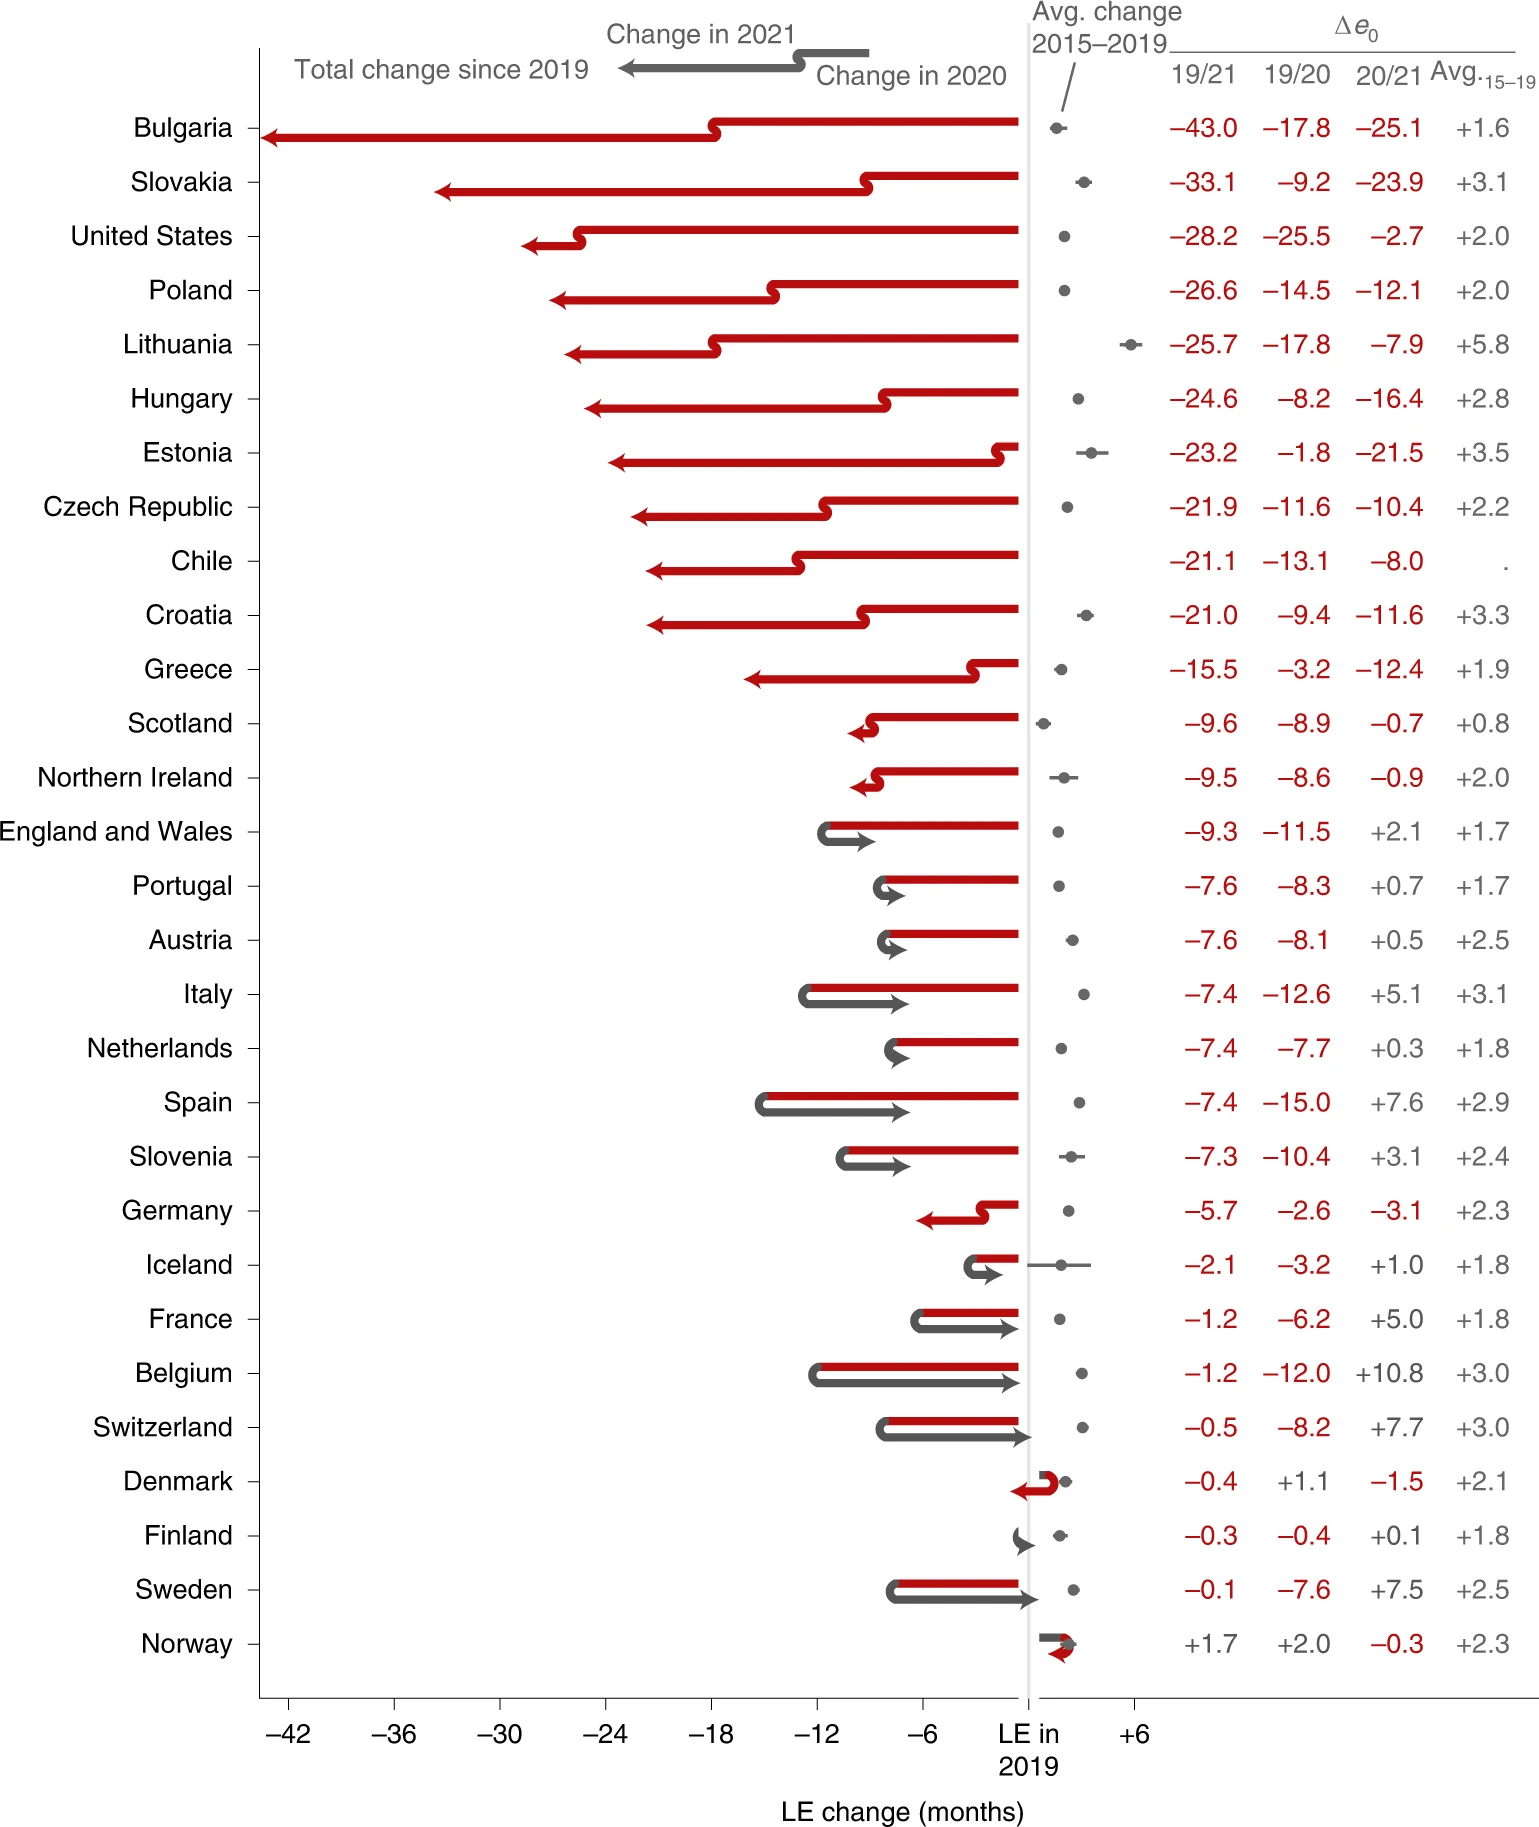
\includegraphics{images/clipboard-211497635.png}

graphique \textbf{Estimating excess mortalityd due to the cvid19
pandemic: a systematic analysis of COVID19 related mortality 2020-2021
Nature} COVID-19 Excess Mortality Collaborators*
\url{https://doi.org/10.1016/} S0140-6736(21)02796-3

Italie très durement touchée

USA aussi mais leader

Innovation qui arrive, l'accès aux soins des Etats unis est le maillon
faible . Le plus troublant encore c'est quand on regarde la carte dans
ce pays qui est un pays fédéral avec les états
républicains/démocrates.\\
Différences fortes entre états républicains/démocrates. On rappelle que
TRump nie l'ampleur de l'épidémoe mais il met 3 milliars de dollars pour
les plateformes vaccinales. Il finance l'innovation.

2 grandes puissances mondailes, ce snot elles qui ont le moins bien
réussi. Quand le prof entend dire que les démocraties sot finies, sont
faibles. Il dit que finalement laréponse des Etats qui ont le moins mal
réussi, ce sont les démocraties européennes, par rapport aux USA et à la
Chine en tout cas.
\end{frame}

\begin{frame}{Bilan COVID en France}
\protect\hypertarget{bilan-covid-en-france}{}
La France est le pays qui a le plus longtemps laissé les écoles
ouvertes.

Estimating the population effectiveness of interventions against
COVID-19 in France A modelling study. Epidemics
\end{frame}

\begin{frame}{Les mesures de restrictions}
\protect\hypertarget{les-mesures-de-restrictions}{}
\begin{itemize}
\item
  Confiement 1: 84\% de réduction de la circulation virale
\item
  Couvre feu
\end{itemize}
\end{frame}

\begin{frame}{France : COVID19 et inégalités en santé}
\protect\hypertarget{france-covid19-et-inuxe9galituxe9s-en-santuxe9}{}
3 graphiques

Distribution de la population résidente de la popualtion hospitalisée
par âge

Distribution de la population par âge (décès et soins critiques)

\begin{tcolorbox}[enhanced jigsaw, rightrule=.15mm, opacityback=0, colframe=quarto-callout-important-color-frame, bottomtitle=1mm, toptitle=1mm, left=2mm, leftrule=.75mm, title=\textcolor{quarto-callout-important-color}{\faExclamation}\hspace{0.5em}{Important}, toprule=.15mm, breakable, colback=white, coltitle=black, opacitybacktitle=0.6, titlerule=0mm, bottomrule=.15mm, colbacktitle=quarto-callout-important-color!10!white, arc=.35mm]

En France, l'accès aux soins s'est fait quand même dans de bonnes
conditions, et plus ou moins égales.

Malgré tout : différence entre les habitants de Sceaux et du 93,
\textbf{8.2 ans de durée de vie de différence}. Facteurs sociétaux,
malbouffe, petits appartements, la drogue, toutce qu'on peut imaginer.\\
\strut \\
Avant le COVID, il y avait déjà une très grande inégalité là-dessus.

Est-ce que la France doit rester avec l'\textbf{égalité de l'accès aux
soins}, ou plutôt \textbf{l'équité de l'accès aux soins} ?
=\textgreater{} Dans les 30 zones où c'est le moins vrai. On ne met
actuellement pas l'offre de soins en prioriété là où il elle serait
nécessaire le plus

\end{tcolorbox}
\end{frame}

\begin{frame}{Conclusions provisoires}
\protect\hypertarget{conclusions-provisoires-1}{}
\begin{enumerate}
\tightlist
\item
  La france consacre une part insuffisante de son PIB à la recherche
  dont l'importance n'est pas comprise par les autorités publiques
  depuis des années. Cette situation est particulirèement visible en cs
  de crise sanitaire.
\end{enumerate}

12 ans pour la création de l'ANRS-MIE à la suite d'une pandémie mondiale
illustre bien une certaine forme d'incompréhension de la part des
décideurs politiques, institutions de recherche, et des chercheurs eux
mêmes vis à vis de la recherche en \ldots.
\end{frame}

\begin{frame}{Chine 2023 : Une crise maeure et prévisible (1)}
\protect\hypertarget{chine-2023-une-crise-maeure-et-pruxe9visible-1}{}
\begin{block}{Quand le politque ne tient pas compte de la
science\ldots{}}
\protect\hypertarget{quand-le-politque-ne-tient-pas-compte-de-la-science}{}
\begin{itemize}
\item
  Janvier 2020: Isolement et séquencage du sarscov2 Transparence
  scientifques
\item
  Février 2020: mise en places du programme 0 covid, Vision politique,
  ils ferment tout. Surveillance par immeuble etc.
\item
  2020-2021 : Stratégie 0 covid qui s'avère effiace (car extrêmement
  dure) + production de vaccins (non mRNA, moins effaces mais portage
  polituque). Est-ce qu'il faut ieux ne pas être dans un pays
  démocratique alors ? vu que ça fonctionne bien ? LE problème c'est que
  leur vaccin fonctionne moins bien, pas mRNA
\item
  2021-2022 : Vaccination des sujets jeunes avec vaccins à efficacité
  réduite, pas de protection des anciens.
\item
  2022 : Arrivée d'OMICRON contenue durant les 6 premiers mois mais avec
  une atteinte majeure aux libertés individuelles. Pour rappel :
  Transmission 1000x supérieure à celui de Wuhan.
\item
  2023 : Echec retentissant de la stratégie 0 covid. La version
  officielle de l'OMS c'est xxx morts, mais y'a probablement eu
  30Milliosn de morts en Chine. Failli exploser en 2022
\end{itemize}
\end{block}
\end{frame}

\begin{frame}{Chine 2023 : Une crise majeure et prévisible (2)}
\protect\hypertarget{chine-2023-une-crise-majeure-et-pruxe9visible-2}{}
\begin{itemize}
\item
  Uene perte de 5 à 7 ans d'espérance de vie
\item
  Un bilan (nombre de décès) ``90 fois supérieur\ldots{}''
\item
  \ldots{}
\item
  \ldots{}
\end{itemize}
\end{frame}

\begin{frame}{France : La réponse du gouvernement à la crise Mars 2020}
\protect\hypertarget{france-la-ruxe9ponse-du-gouvernement-uxe0-la-crise-mars-2020}{}
\begin{enumerate}
\tightlist
\item
  La création d'un conseil scientifique indépendant de novo -- 9 mars
  2020
\item
  Conseil de défense Covid-19
\item
  La promulgation de la loi d'urgence n9 2020-290 du 23 mars 2020 pour
  faire face à l'épidémoe de covid10 ui permettant de prendre ds
  décisiosn opérationnelles et de les faire valdier par le Parlement
  dans un 2ème temps
\item
  La recherche d'une politique européenne cordoonnée -- fin mars
\end{enumerate}
\end{frame}

\begin{frame}{Fonctionnement du Conseil scientifique COVID-19}
\protect\hypertarget{fonctionnement-du-conseil-scientifique-covid-19}{}
\begin{enumerate}
\setcounter{enumi}{1}
\tightlist
\item
  TEmporalité n'est pas la même

  \begin{itemize}
  \tightlist
  \item
    Temps des médias : heures
  \item
    Temps des plitiques : jours
  \item
    Temps ds scientifuqes : mois
  \end{itemize}
\item
  Doute, incertitude, modestie et humilité

  \begin{itemize}
  \tightlist
  \item
    La science se construit sur le doute teoutefois les polituques
    n'aiment pas le doute. dans la haute hiérarchie les décideurs n'ont
    pas à faire de thèses (différente de l'allemagne). ``Ce sont de
    machines à décider, on les formes à décider à trancher. On ne leur
    apprend pas à écouter. Ils sont formés de façon différente.''
  \end{itemize}
\item
  Anticipation

  \begin{itemize}
  \tightlist
  \item
    \textbf{Une grande évolution}
  \item
    Le fait que la courbe épidémique soit exponentelle montre qu'il est
    nécessaires d'naticiper pour ne pas saturer le sytème de soins. 3
    messages d'anticipation plus ou moins perçus
  \end{itemize}
\item
  Agenda

  \begin{enumerate}
  \setcounter{enumii}{1}
  \item
    Les politiques et les cientifiques n'ont pas les mêmes agendas :

    Les premiers \ldots{} et les seconds\ldots{}
  \end{enumerate}
\end{enumerate}
\end{frame}

\begin{frame}{Fonctionnement du Conseil scientifique COVID-19 et
autorités}
\protect\hypertarget{fonctionnement-du-conseil-scientifique-covid-19-et-autorituxe9s}{}
3 niveaux de relations avec les autorités
\end{frame}

\begin{frame}{Quelques moments clefs entre le CV et les politques}
\protect\hypertarget{quelques-moments-clefs-entre-le-cv-et-les-politques}{}
12 mars 2020 : réunion à l'élysée. Décision du 1er confinement

9 avril 2020 : Visite de l'IHU Marseille. Le prof raconte qu'il essaie
de dire au Président qu'il ne faut pas aller à MArseille pour ne pas
donner du crédit à Raoult mais il peut pas lutter logntemps donc ils y
vont. Il veut pas donner son avis au président pour pas l'influencer et
le président se fait son avis. Ensuite le président lui dit qu'il s'est
fait son avis, le prof a gagné sur le fond mais par contre il se fait
défoncer par le conseil scientifique qui lui dit qu'il aurait jamais dû
aller là-bas, ce avec quoi il était d'accord detoute façon.

28 septembre 2020 : Annonce au gouvernement de la nécessité d'un 2ème
confinement qui sera mis en place seulement fin octobre 2020

28 novembre 2020 : stratégie vaccinale

26 janvier 2021 : Annonces du gvt de la nécessité d'un 3ème confinement
qui ne sera mis en place qu'en avril 2021.

mai 2021 : LEs vaccins mRNA protegent ils contre
l'infection/transmission ?

5 juin 2021 : choix d'un pass sanitaire par rapport au pass vaccinal

15 décembre 2021 : Omicron. Annonce au gouvernement de l'explosion des
contaminations en janvier 2022 mais le systèe de santé ..
\end{frame}

\begin{frame}{Transparence, Comité citoyen}
\protect\hypertarget{transparence-comituxe9-citoyen}{}
\begin{block}{Appel à la responsabilité et aux choix personnelles et
volontaires}
\protect\hypertarget{appel-uxe0-la-responsabilituxe9-et-aux-choix-personnelles-et-volontaires}{}
Mettre en margin droit Quarto l'image de la couverture du livre ``Il
faut défendre la société'' de Michel Foucault. Cours au collège de
France

\begin{itemize}
\item
  Une volonté de tarnsparence: publication d'avis et de notes, auditions
  par l'Assemblée nationale, le Sénat, le Conseil économique, social et
  environnemental (CESE), la commission Pittet, interventosn dans la
  presse ..
\item
  Un appel à la création d'un comité citoyen, porté par le conseil
  Scientifique, la Comission nationale de la anté et la Comission
  nationale des droits de l'homme =\textgreater{} finalement ça ne s'est
  pasfait. Dans le contexte en confiance entre le peuple et les
  politques, ça aurait été bien pourtant. Il y a eu largement une
  relatio Top/Down. Pour le prof c'est un grand échec.
\item
  Un échec au niveau national mais un succès au niveau des grandes
  métropoles (Grenoble Lyon Bordeaux Paris sTrasbourg)
\item
  Une doctrine constante de resposnabilitéet de choix personnes des
  citoyens.\\
  Des choix volontaires pour chaque mesure : écoles, tests, isolement
  après la fin du confinement pour les patients positifs ou les patients
  âgés à haut risque\ldots{}
\item
  Mais aussi une recommandation forte pour le passe sanitaire et en
  juillet 2021, la vaccination obligatoire de ssoignantes
\item
  L'introduction du rappel vaccinal dans le passe sanitaire (novembre

  \begin{enumerate}
  [1)]
  \setcounter{enumi}{2020}
  \tightlist
  \item
  \end{enumerate}
\end{itemize}

Le prof regrette que l'explicaton ne se soit pas faite (par cause de la
formation des énarques probablmenet) longuement comme ça a pu être le
cas dans d'autres pays. JE crois qu'il a pris l'exemple de la Finlande
ou de la Hollande.
\end{block}
\end{frame}



\end{document}
